\documentclass{article}
\usepackage[utf8]{inputenc}
\usepackage[russian,english]{babel}
\usepackage{graphicx}
\usepackage{colortbl}
\usepackage{multicol}
\usepackage{graphicx}
\graphicspath{ {./images/} }

\newcommand{\VK}[1]{{\color{orange} {\bf (VK: #1)}}}

\title{A closer look at the impact of activation functions on Generalizability}
\author{ Gabriela Tsvetkova
 
 \\ gabriellatsvetkova43@gmail.com \and  Under the guidance of Victor Kolev \\ Stanford University
 }
\date{ \\ 2020}

\usepackage{biblatex}
\addbibresource{reference.bib}

\usepackage{csquotes}

\usepackage{url}
\usepackage{hyperref}
\usepackage{amsmath}
\usepackage{booktabs}
\usepackage{amsfonts}
\usepackage{amssymb}
%\usepackage{amsthm}
\usepackage{array}
\usepackage{todonotes}
%\usepackage{tabularx}
%\usepackage{natbib}
\usepackage{pgf,tikz,pgfplots}
\pgfplotsset{compat=1.15}
\usepackage{bm}
\usepackage{mathrsfs}
%\usepackage{tabulary}
\usetikzlibrary{arrows}
\usetikzlibrary[patterns]


\begin{document}

\maketitle
% \begin{abstract}



%\end{abstract}


\newpage

\renewcommand{\contentsname}{Content}

\tableofcontents

\newpage
\section{Introduction}


Over the past decades, an overwhelming body of research has been constituting the effectiveness of Deep Learning. These black-box models - neural networks - are not explicitly programmed for a particular task, instead an ability to optimize their performance is implemented. They do so as they gain experience starting from zero, and gradually acquire potential for recognizing certain patterns.

Neural networks are basically a complex composition of affine transformations. However, linearity does not give the model the capacity needed to approximate any function given unlimited data and infinite time for training. That is why non-linear activation functions such as Sigmoid, Tanh, ReLU are introduced to the problem. 

A recent paper \cite{SiNU} showed that using $y = sin(x)$ as an activation function keeps the structure of the training examples because $\frac{d^n}{d\ x^n} \sin(\theta) = \cos(\theta) , n \in \mathbb{N} $.

In this paper we investigate the influence of 3 activation functions while training the models to approximate fundamental mathematical functions such as $y = x^2$ and $y = x^3$. Empirically, it can be inferred that activation functions implement explicit structures in the network, which biases training towards functions similar to the activation first derivatives. 

This work paves way for research into the inductive biases of neural network design, which if properly exploited could improve network stability, training speed, generalization, and applicability. 


\section{Concepts}
   \label{Background}
   
    \subsection{Feedforward neural network}
    A feedforward neural network consists of nodes and connections between them. Each neuron is associated with an activation and a bias and each connection -- with a certain weight.
   
    The value of the activation function of the neurons in layer $l$ is obtained by the following formula:
    
     $$\bm a^{(l)} = g(\bm W^{(l)} \bm a^{(l-1)} + \bm b^{(l)})$$
     
    Here, $n_l$ is the number of units in layer $l$; $\bm a^{(l)} \in \mathbb{R}^{n_l}$ is the vector containing the activations of the neurons in layer $l$; $\bm W^{(l)} \in \mathbb{R}^{n_l \times n_{l-1}}$ is the matrix containing the weights which connect the neurons in layer $l$ to those in layer $l-1$; $\bm b^{(l)} \in \mathbb{R}^{n_l}$ is the vector containing the biases of the neurons in layer $l$; and $g$ is some non-linear activation function.
    
   \subsection{Loss function}
    
    The loss function evaluates how well specific algorithm models the given data i.e. the error. Since we are working in a continuous domain, we use the mean square error function:
    
    $$\mathcal{L} = \frac{1}{n_L}\|\bm y - \bm a^{(L)}\|^2$$
    
    Here, $\bm y \in \mathbb{R}^{n_L}$ is the vector containing the ground truth outputs; $\bm a^{(L)} \in \mathbb{R}^{n_L}$ is the vector containing the activations of the neurons in the last layer ($L$) i.e. the vector containing the predictions; and $\|.\|$ is the Euclidean norm.   
    Two algorithms are involved in the process of learning of the neural network -- backpropagation and gradient descent. For the latter we use Adam \cite{adam} in our experiments.
    
\section{Methods}
\label{Methods}

    \subsection{Activation Functions}
    In this paper the activation functions used are as follows:
    ReLU, Tanh, Leaky ReLU, and SiNU:
    
    $$ \ \ \ \text{ReLU}(x) = \begin{cases} 
                    0 & x \leq 0 \\
                    x & x > 0 \\
                 \end{cases}$$
    
    $$\text{Leaky ReLU}(x) = \begin{cases} 
                    0.01x & x \leq 0 \\
                    x & x > 0 \\
                 \end{cases}$$
    $$\ \text{Tanh}(x) = \frac{e^x - e^{-x}}{e^x + e^{-x}}$$
    
    $$\ \ \ \ \text{SiNU}(x) = sin(x)$$
    %Mention SiNAR paper
    
    \subsection{Spectral Norm Regularization}
    
    Neural networks tends to learn the training examples well, but fail to generalize to new examples. This is known as overfitting, and stems from the fact that the minimum error objective is ill-posed. For instance, the Lagrange polynomial of a set of points would have the smallest loss, yet it would not have high generalization error.
    
    One method of alleviating overfitting is regularization. This is the process of penalizing big values in the weight matrix with the effect of a model which adapts well to new data.  
    
    In this paper we focus on Spectral Norm Regularization. \cite{spectral}. The motivation behind it is due to (Neyshaubar etal 2019)\cite{Neyshaubar} and \cite{Arora}. The spectral norm of a matrix W $ \in \mathbb{R}^ {m\times n} $ is the largest singular value of it and it is defined as: 
    $$\sigma = \max_{\xi \in \mathbb{R}^ {n}, \xi \neq 0}\dfrac{ \|A\xi\|_2}{\|\xi\|_2}$$
    
    
    

\section{Results}
\label{Results}
We use fully-connected layers as size, range, activation function, spectral norm regularization coefficient. 
In the graphs below are shown the models with the best performance on the two tasks.

\begin{figure*}[h!]
\begin{multicols}{2}
    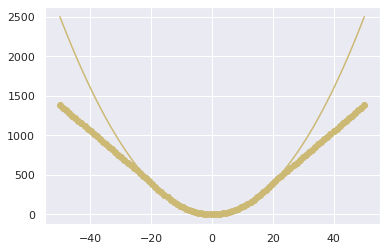
\includegraphics[width=\linewidth]{ReLUx2.png}\par 
    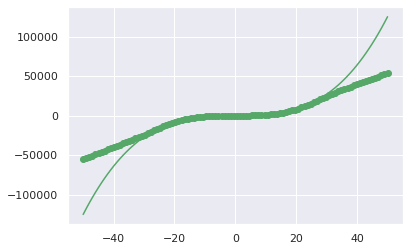
\includegraphics[width=\linewidth]{ReLUx3.png}\par 
\end{multicols}
\caption{The left graph shows a model that approximates $y = x^2$ trained on range [-20;20] with ReLU. It is visible that the graph of the objective function keeps a linear structure because of its activation function. The same can be inferred for the right graph of $y=x^3$. }
\begin{multicols}{2}
    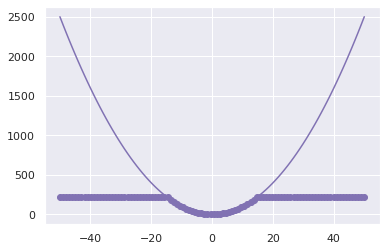
\includegraphics[width=\linewidth]{Tanhx2.png}\par
    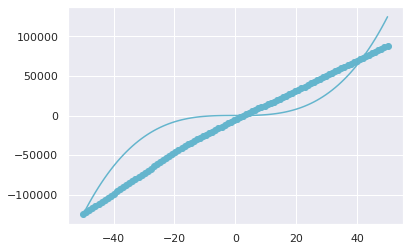
\includegraphics[width=\linewidth]{Tanhx3.png}\par
\end{multicols}
\caption{The left graph shows a model that approximates $y = x^2$ trained on range [-20;20] with Tanh. It is visible that the graph of the objective function keeps a linear structure because of its activation function. The same can be inferred for the right graph of $y=x^3$.}
\end{figure*}


\begin{figure*}[h!]
\begin{multicols}{2}
    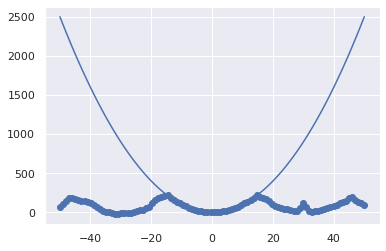
\includegraphics[width=\linewidth]{x2_SiNU.png}\par
    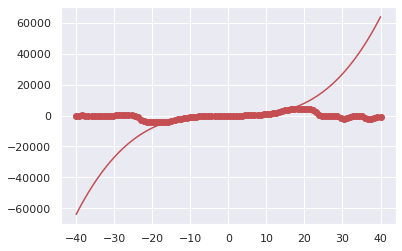
\includegraphics[width=\linewidth]{x3_SiNU.png}\par
\end{multicols}
\caption{The left graph shows a model that approximates $y = x^2$ trained on range [-20;20] with SiNU. It is visible that the graph of the objective function keeps a linear structure because of its activation function. The same can be inferred for the right graph of $y=x^3$.}
\end{figure*}
\newpage

% \begin{figure}
%     \centering
%     \includegraphics[scale=0.3]{example-image}
%     \caption{Your caption}
% \end{figure}

\section{Future Development}
\label{Future Work}
Experiments such as changing the range of input data, type of function, the architecture of the neural network and the type of regularization Dropout\cite{dropout} are always interesting and may lead to better understanding of the impact of activation functions.
A further investigation with modular neural networks \cite{gnn} for composing complex functions can be made.


\section{Conclusion}
\label{Conclusion}

\printbibliography
\end{document}